A company specialising in food supplements production for some animals wanted to conduct an experiment with the main aim of figuring out whether a slight decrease in the recommended dosages of three particular products taken together would make a significant impact on the resulting ``performance'', which is expressed in terms of some continuous response. The dosage range of interest for each supplement is from $90\%$ to $100\%$ of the standard recommendation; it is desired that there would be $3$ levels (i.e. taking the values of $90\%$, $95\%$ and $100\%$). Carrying out the experiment with more than $3$ levels was possible but more complicated, as measuring, for example, $92.5\%$ of the recommended dosage might be quite tricky. However, the search was performed among a larger $5$-level candidate set of points (which, obviously, contains all $3$-level design points), but due to the form of the fitted model and the criteria used, the resulting designs' points consist of only $3$-level points.

In total such treatments are to be applied to $36$ cages of animals, which would be allocated in $2$ equal sized blocks. The response surface model, therefore, would contain all linear, quadratic and interaction terms, so, since there are $3$ factors, the number of terms in the fitted model is $p=9$.  However, there were some doubts regarding the expected curvature of the fitted function, in other words, the presence of third-order terms was anticipated: a linear-by-linear-by-linear term, quadratic-by-linear and cubic terms ($q=10$ overall). 

Another restriction was that the experimenters wanted to have at least two centre points in each block to ensure representation of the conditions thought a priori most likely to be best (with dosages of $95\%$ for each supplement), i.e. $4$ runs in total were fixed beforehand; this constraint was built directly into the search procedure.

\subsection{Design search}

Taking into account the possibility of the fitted second-order polynomial providing not the best fit, and the true relationship between the response and the dosages being influenced by the third-order terms, we can express this in terms of the full model
\begin{equation*}
\bm{Y}=\bm{Z\beta}_{B}+\bm{X}_{1}\bm{\beta}_{1}+\bm{X}_{2}\bm{\beta}_{2}+\bm{\varepsilon},
\end{equation*}
and the fitted model: 
\begin{equation*}
\bm{Y}=\bm{Z\beta}_{B}+\bm{X}_{1}\bm{\beta}_{1}+\bm{\varepsilon},
\end{equation*}
where $\bm{\varepsilon}\sim \mathcal{N}(\bm{0},\sigma^{2}\bm{I}_{n}).$

The notation here and further on is the same as before:
\begin{itemize}
\item $\bm{X}_{1}$ -- model matrix of primary terms
\item $\bm{\tilde{X}}_{1}=[\bm{Z},\bm{X}_{1}]$, where columns of $\bm{Z}$ contain block indicators
\item $\bm{X}_{2}$ -- model matrix of potential terms
\item $\bm{\tilde{M}}=\bm{X}'_{1}\bm{Q}\bm{X}_{1}$, $\bm{Q}= \bm{I}_{n}-\bm{Z}(\bm{Z}'\bm{Z})^{-1}\bm{Z}'$
\item $\bm{\tilde{L}}=\bm{X}'_{2}\bm{X}_{2}-\bm{X}'_{2}\bm{\tilde{X}}_{1}(\bm{\tilde{X}}'_{1}\bm{\tilde{X}}_{1})^{-1}\bm{\tilde{X}}'_{1}\bm{X}_{2}$ -- dispersion matrix, and 
\item $\bm{\tilde{A}}= (\bm{\tilde{X}}'_{1}\bm{\tilde{X}}_{1})^{-1}\bm{\tilde{X}}'_{1}\bm{X}_{2}$ -- alias matrix for the blocked model.
\end{itemize}

The experimenters preferred using the determinant-based criterion as the primary inferential interest is on the overall input of the model terms. Together with good precision of the parameters to be estimated ($\bm{\beta}_1$), other objectives are to minimise the impact of the potential terms' possible presence and the bias and variance of the primary terms' estimators.
 
Hence it was decided to optimise the mean square error based criterion function, in the same form as it was derived in (\ref{eq::MSE_D_B}):
\begin{align}
\label{eq::crit1}
&\left[\left|\bm{\tilde{M}}\right|^{-1/p}F_{p,d_B;1-\alpha_{\!_{DP}}}\right]^{\kappa_{\!_{DP}}} \times \notag \\ &\left[\left|\bm{\tilde{L}}+\frac{\bm{I}_{q}}{\tau^{2}}\right|^{-1/q}F_{q,d_B;1-\alpha_{\!_{LoF}}}\right]^{\kappa_{\!_{LoF}}}\times \notag\\ & \left[|\bm{\tilde{M}}|^{-1}\exp\left(\frac{1}{N}\sum_{i=1}^{N}\log(1+\bm{\tilde{\beta}}_{2i}'\bm{X}_2^{'}\bm{Q}\bm{X}_1\bm{\tilde{M}}^{-1}\bm{X}_1^{'}\bm{Q}\bm{X}_2\bm{\tilde{\beta}}_{2i})\right)\right]_{.}^{\kappa_{\!_{MSE}}/p}
\end{align}

Recall that here $d_B$ is the number of pure error degrees of freedom for the blocked experiment, as was described in Section \ref{sec::back_blocked}. 

Although the primary choice of the number of levels of each factor is $3$, the number of experimental runs would allow for $5$ levels so that all of the potential terms can be estimated. So we considered one more compound criterion which has a different lack-of-fit component: $DP_S$-- optimality for potential terms in the full (third-order polynomial) model, arising from the $D_S$-optimality that was suggested by \cite{Atkinson2007} (page $360$) in the context of model discrimination:
\begin{align}
\label{eq::crit2}
&\left[\left|\bm{\tilde{M}}\right|^{-1/p}\mathrm{F}(p,d,\alpha_{\!_{DP}})\right]^{\kappa_{\!_{DP}}} \times  \left[|\bm{\tilde{L}}|^{-1/q}F_{q,d_B;1-\alpha_{LoF}}\right]^{\kappa_{\!_{LoF}}}\times \notag\\ & \left[|\bm{\tilde{M}}|^{-1}\exp\left(\frac{1}{N}\sum_{i=1}^{N}\log(1+\bm{\tilde{\beta}}_{2i}'\bm{X}_2^{'}\bm{Q}\bm{X}_1\bm{\tilde{M}}^{-1}\bm{X}_1^{'}\bm{Q}\bm{X}_2\bm{\tilde{\beta}}_{2i})\right)\right]_{.}^{\kappa_{\!_{MSE}}/p}
\end{align}

This criterion further on will be referred to as the ``full'' criterion, and we shall explore how this would affect the resulting designs.

Regarding the parameters of the criteria function, they need to be determined for the design search:
\begin{itemize}
\item $\tau^2$ is the scaling parameter of the variance of the potential terms such that $\bm{\beta}_2\sim \mathcal{N}(\bm{0},\tau^{2}\sigma^{2}\bm{I}_{q})$ and $\bm{\tilde{\beta}}_2\sim \mathcal{N}(\bm{0},\tau^{2}\bm{I}_{q})$. For each criterion we will consider two cases: $\tau^2=1$ and $\tau^2=1/q$. 
\item $N$ is the number of Monte Carlo samples used to estimate the third criterion component. For $\tau^2=1$ $N=500$, and for $\tau^2=1/q$ we set $N=1000$ in order to have a sufficiently small relative estimation error.
\item The number of random starts in the point exchange algorithm is set to $50$.  
\end{itemize}

One of the pre-specified requirements was the presence of at least two centre points in each block. In order to implement that, the point exchange algorithm was slightly amended: at each random initial non-singular designs the first two points in each block are set to be centre points, and every loop with the exchange steps would then start from the third point onwards, so that whatever changes are to be accepted by the algorithm, it would always keep these two points; such an amendment  actually reduced a bit the number of exchanges to be performed. 

For the sake of assessing the quality of the designs obtained with this restriction, we will obtain also designs without any and will evaluate the efficiency losses.

\subsection{Results}

In this section we will give a summary of the designs we looked at while searching for the best one for this particular experimental setup. We considered three schemes of weight allocations: the first one is with the weight being equally distributed between the components, the second one -- with a bit more weight ($0.4$) put on minimising the variation of the primary terms' estimators and their bias, with the rest allocated to the lack-of-fit component. The third one has half of the weight on the $MSE$-component with the rest of it distributed evenly among the other two components. For the sake of reference we also provided the performances of the $DP$-, $LOF(DP)$- and $MSE(D)$-optimal designs (\#$4$ -- \#$6$ in the tables below). 

Table \ref{tab::MSE(D)_case} provides the performances of the optimal designs with respect to the criteria given in (\ref{eq::crit1}), without forcing the presence of two centre points per block. The main feature observed is that in general individual efficiency values are quite large (especially in comparison to the previously seen example); this might be explained by the fact that the number of available residual degrees of freedom ($n-b-p=25$) is quite large compared to the number of primary terms ($p=9$) that are to be estimated, and this flexibility results in better compromises achievable between the three criterion components.

%%% MSE(D)-optimal designs, WITHOUT centre points: DP, LoF(DP) and MSE(D)

\begin{table}[h]
\centering
\caption{Case-study. Properties of MSE(D)-optimal blocked designs}
\label{tab::MSE(D)_case}
\scalebox{0.75}{
%\resizebox{\textwidth}{!}}                               \\
   & \textbf{DP}       & \textbf{LoF(DP)}    & \textbf{MSE(D)}   & \textbf{PE}        & \textbf{LoF}        & \textbf{DP}   & \textbf{LoF(DP)}   & \textbf{MSE(D)} \\
1 & 1/3  & 1/3  & 1/3 & \multicolumn{1}{|r}{16} & \multicolumn{1}{r|}{9}  & 90.58  & 95.60  & 97.34  \\
2 & 0.4  & 0.2  & 0.4 & \multicolumn{1}{|r}{16} & \multicolumn{1}{r|}{9}  & 93.09  & 89.23  & 98.68  \\
3 & 0.25 & 0.25 & 0.5 & \multicolumn{1}{|r}{14} & \multicolumn{1}{r|}{11} & 89.10  & 94.04  & 99.52  \\
4 & 1    & 0    & 0   & \multicolumn{1}{|r}{21} & \multicolumn{1}{r|}{4}  & 100.00 & 71.70  & 98.84  \\
5 & 0    & 1    & 0   & \multicolumn{1}{|r}{14} & \multicolumn{1}{r|}{11} & 64.62  & 100.00 & 76.95  \\
6 & 0    & 0    & 1   & \multicolumn{1}{|r}{8}  & \multicolumn{1}{r|}{17} & 69.48  & 75.00  & 100.00 \\
 & & & & & & & & \\
   & \multicolumn{3}{l}{\textbf{Criteria, $\bm{\tau^2=1/q}$}} & \multicolumn{2}{l}{\textbf{DoF}} & \multicolumn{6}{l}{\textbf{Efficiency, \%}}                               \\
   & \textbf{DP}       & \textbf{LoF(DP)}    & \textbf{MSE(D)}   & \textbf{PE}        & \textbf{LoF}        & \textbf{DP}   & \textbf{LoF(DP)}   & \textbf{MSE(D)} \\
1 & 1/3  & 1/3  & 1/3 & \multicolumn{1}{|r}{21} & \multicolumn{1}{r|}{4}  & 100.00 & 99.90  & 98.70  \\
2 & 0.4  & 0.2  & 0.4 & \multicolumn{1}{|r}{21} & \multicolumn{1}{r|}{4}  & 99.64  & 99.71  & 98.88  \\
3 & 0.25 & 0.25 & 0.5 & \multicolumn{1}{|r}{21} & \multicolumn{1}{r|}{4}  & 100.00 & 99.90  & 100.53 \\
4 & 1    & 0    & 0   & \multicolumn{1}{|r}{21} & \multicolumn{1}{r|}{4}  & 100.00 & 98.57  & 99.83  \\
5 & 0    & 1    & 0   & \multicolumn{1}{|r}{21} & \multicolumn{1}{r|}{4}  & 86.31  & 100.00 & 87.26  \\
6 & 0    & 0    & 1   & \multicolumn{1}{|r}{8}  & \multicolumn{1}{r|}{17} & 69.38  & 72.21  & 100.00
\end{tabular}
}
\end{table}

Now we introduce the compulsory centre points, and see how the resulting designs perform. Table \ref{tab::MSE(D)_caseCP} contains two types of efficiencies: ``Global'' efficiencies are calculated with respect to the optimal designs obtained without any fixed points, whilst ``Local'' efficiencies compare the obtained designs with the best designs among the blocked designs with at least two centre points per block. The latter ones will be, obviously, larger, and the differences between the two for the same components represent the measure of the loss by restricting the set of designs to be considered. The last column of this table, ``Relative Efficiency,'' is essentially the efficiency of a given design with respect to the optimal one in terms of the same compound criterion (i.e. with the same allocation of weights), obtained without any restrictions; this value gives a ``single-value'' perspective on the efficiency loss.  

%%% MSE(D)-optimal designs, WITH centre points: DP, LoF(DP) and MSE(D)

\begin{table}[h]
\caption{Case-study. Properties of MSE(D)-optimal blocked designs, with two centre points per block}
\label{tab::MSE(D)_caseCP}
\resizebox{\textwidth}{!}}  & \multicolumn{3}{l}{\textbf{`Local' Efficiency,\%}}& \multicolumn{1}{c}{\textbf{Relative}}                          \\
   & \textbf{DP}       & \textbf{LoF(DP)}    & \textbf{MSE(D)}   & \textbf{PE}        & \textbf{LoF}        & \textbf{DP}   & \textbf{LoF(DP)}   & \textbf{MSE(D)}  &  \textbf{DP}       & \textbf{LoF(DP)}   & \textbf{MSE(D)} & \textbf{Efficiency,\%} \\
1 & 1/3 & 1/3 & 1/3 & \multicolumn{1}{|r}{14} & \multicolumn{1}{r|}{11} & 88.63 & 90.03 & 99.97 & \multicolumn{1}{|r}{92.89} & 97.59 & \multicolumn{1}{r|}{100.75} & 98.18 \\
2 & 0.4 & 0.2 & 0.4 & \multicolumn{1}{|r}{14} & \multicolumn{1}{r|}{11} & 88.35 & 90.14 & 99.15 & \multicolumn{1}{|r}{92.60} & 97.70 & \multicolumn{1}{r|}{99.92} & 98.31 \\
3 & 0.25 & 0.25 & 0.5 & \multicolumn{1}{|r}{14} & \multicolumn{1}{r|}{11} & 88.63 & 90.03 & 99.75 & \multicolumn{1}{|r}{92.89} & 97.59 & \multicolumn{1}{r|}{100.53} & 98.90 \\
4 & 1 & 0 & 0 & \multicolumn{1}{|r}{20} & \multicolumn{1}{r|}{5} & 95.41 & 62.13 & 95.24 & \multicolumn{1}{|r}{100.00} & 67.34 & \multicolumn{1}{r|}{95.98} & 95.58 \\
5 & 0 & 1 & 0 & \multicolumn{1}{|r}{14} & \multicolumn{1}{r|}{11} & 66.49 & 92.26 & 79.91 & \multicolumn{1}{|r}{69.69} & 100.00 & \multicolumn{1}{r|}{80.53} & 92.26 \\
6 & 0 & 0 & 1 & \multicolumn{1}{|r}{14} & \multicolumn{1}{r|}{11} & 88.31 & 88.35 & 99.23 & \multicolumn{1}{|r}{92.55} & 95.77 & \multicolumn{1}{r|}{100.00} & 99.23 \\
 & & & & & & & & & & & & \\
   & \multicolumn{3}{l}{\textbf{Criteria, $\bm{\tau^2=1/q}$}} & \multicolumn{2}{l}{\textbf{DoF}} & \multicolumn{3}{l}{\textbf{`Global' Efficiency,\%}}  & \multicolumn{3}{l}{\textbf{`Local' Efficiency,\%}}& \multicolumn{1}{c}{\textbf{Relative}}                          \\
   & \textbf{DP}       & \textbf{LoF(DP)}    & \textbf{MSE(D)}   & \textbf{PE}        & \textbf{LoF}        & \textbf{DP}   & \textbf{LoF(DP)}   & \textbf{MSE(D)}  &  \textbf{DP}       & \textbf{LoF(DP)}   & \textbf{MSE(D)} & \textbf{Efficiency,\%} \\
1 & 1/3 & 1/3 & 1/3 & \multicolumn{1}{|r}{18} & \multicolumn{1}{r|}{7} & 92.52 & 95.13 & 95.86 & \multicolumn{1}{|r}{96.97} & 98.00 & \multicolumn{1}{r|}{96.55} & 94.95 \\
2 & 0.4 & 0.2 & 0.4 & \multicolumn{1}{|r}{18} & \multicolumn{1}{r|}{7} & 94.19 & 92.19 & 96.54 & \multicolumn{1}{|r}{98.72} & 94.98 & \multicolumn{1}{r|}{97.24} & 95.34 \\
3 & 0.25 & 0.25 & 0.5 & \multicolumn{1}{|r}{17} & \multicolumn{1}{r|}{8} & 92.44 & 93.70 & 97.05 & \multicolumn{1}{|r}{96.88} & 96.53 & \multicolumn{1}{r|}{97.75} & 95.72 \\
4 & 1 & 0 & 0 & \multicolumn{1}{|r}{20} & \multicolumn{1}{r|}{5} & 95.41 & 90.63 & 95.66 & \multicolumn{1}{|r}{100.00} & 93.37 & \multicolumn{1}{r|}{96.35} & 95.41 \\
5 & 0 & 1 & 0 & \multicolumn{1}{|r}{22} & \multicolumn{1}{r|}{3} & 76.11 & 97.07 & 77.10 & \multicolumn{1}{|r}{79.77} & 100.00 & \multicolumn{1}{r|}{77.65} & 97.07 \\
6 & 0 & 0 & 1 & \multicolumn{1}{|r}{14} & \multicolumn{1}{r|}{11} & 88.37 & 90.37 & 99.29 & \multicolumn{1}{|r}{92.62} & 93.10 & \multicolumn{1}{r|}{100.00} & 99.29
\end{tabular}
}
\end{table}

The first observation to be made here is that the imbalance in the distribution of the residual degrees of freedom is not as strong as in the unrestricted case. However, the prevalence towards the pure error degrees of freedom is still evident. Designs' efficiencies in terms of individual components are still quite large, both ``local'' and ``global'' ones. In general, the performances are better for smaller $\tau^2$ (except for the $MSE(D)$ part), as in this case the model disturbance effect is assumed to be quite small, and the compromise might be more feasible. Overall, relative efficiencies are quite good, losses among the first three designs (optimal with respect to the compound criteria) do not exceed $1.82\%$ for $\tau^2$ and $5.05\%$ for $\tau^2=1/q$.

It is notable that designs \#$1$ and \#$3$ (for the larger $\tau^2$) are the same. Its $MSE(D)$-value turned out to be better than of the design \#$6$, which was constructed as being optimal with respect to this component. This design was chosen to be used when carrying out the experiment; the experiment was run successfully and useful conclusions were drawn from the obtained data. The design can be found in Table \ref{tab::CS_Design} below, the points in each block have been ordered for the sake of easier perception, and, of course, they have to be and were randomised in each block before running the experiment.

\begin{table}[h]
\caption{Case-study. MSE(D)-optimal design \#$1$ with two centre points, $\tau^2=1$}
\begin{center}
\label{tab::CS_Design}
\scalebox{0.73}{
%\resizebox{\textwidth}{!}{%
\begin{tabular}{rrrrrrr}
-1 & -1 & -1 &  & -1 & -1 & -1 \\
-1 & -1 & 0  &  & -1 & -1 & 0  \\
-1 & -1 & 1  &  & -1 & -1 & 1  \\
-1 & 0  & -1 &  & -1 & 0  & 1  \\
-1 & 1  & -1 &  & -1 & 1  & -1 \\
-1 & 1  & 1  &  & -1 & 1  & 0  \\
-1 & 1  & 1  &  & 0  & -1 & -1 \\
0  & -1 & 1  &  & 0  & -1 & 1  \\
0  & 0  & 0  &  & 0  & 0  & 0  \\
0  & 0  & 0  &  & 0  & 0  & 0  \\
0  & 1  & -1 &  & 0  & 1  & 1  \\
1  & -1 & -1 &  & 1  & -1 & -1 \\
1  & -1 & 0  &  & 1  & -1 & 0  \\
1  & -1 & 1  &  & 1  & -1 & 1  \\
1  & 0  & 1  &  & 1  & 0  & -1 \\
1  & 1  & -1 &  & 1  & 0  & 1  \\
1  & 1  & 0  &  & 1  & 1  & -1 \\
1  & 1  & 1  &  & 1  & 1  & 1 
\end{tabular}
}
\end{center}
\end{table}

\begin{figure}[h]
\begin{center}
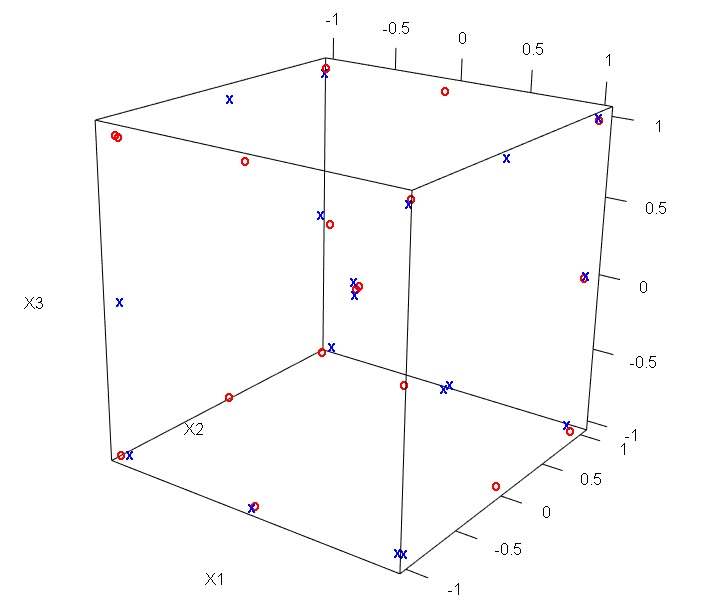
\includegraphics[scale=0.65]{CS_design.jpg}      %width=\textwidth
\caption{MSE(D)-optimal design \#$1$ with two centre points, $\tau^2=1$}
\label{fig::CS_design}
\end{center}
\end{figure} 

Figure \ref{fig::CS_design} provides a graphical representation of the design: the three axes correspond to the experimental factors, each is at three levels (i.e. scaled to $[-1,1]$ dosages): $-1$, $0$ and $1$. Each dot is a design point, and two colours (blue and red) and two symbols (`x' and `o') serve as block indicators. We can see that there are only two centre points in each block, as required, and replicates of other points are generally split between blocks (except for the $(-1,1,1)$ point which is duplicated in the first block only). 

All other designs may be found in the Supplementary material. Time-wise, for the search algorithm's parameters outlined in the beginning of this section, on average an optimal design was found in $13-15$ hours, which was acceptable in this particular case. Sometimes, however, it took up to $20-24$ hours, so some extra time allowance should be accounted for when using these criteria and this search algorithm. 

%%% MSE(D)-optimal designs, WITH centre points: DP, LoF(DPs) and MSE(D) -- LoF as Ds for potential terms
Further we decided to check what designs we would get if there were $5$ levels of each factor rather than $3$, so that all of the third-order terms are estimable (which is also feasible due to a large enough number of runs), i.e. the lack-of-fit component minimising the posterior confidence region for the potential terms would be replaced by the $DP_S$-optimality for them, as in (\ref{eq::crit2}). 

The summary of the corresponding optimal designs is given in Table \ref{tab::MSE(D)_caseCPLoF}: the `new' lack-of-fit component is denoted by DP*s. The notions of `global'  and `local' efficiencies are the same as previously. For each design we calculated its $LoF(DP)$-value, so that we could assess how they would perform in terms of the criterion (\ref{eq::crit1}). The performances of the optimal designs constructed without the restriction of two centre points per block are summarised in Table \ref{tab::MSE(D)_full} in Appendix \ref{app::cs}; all of the designs are also provided in the Supplementary material. In order to illustrate general tendencies in the designs' appearances, designs optimal with respect to the criterion with equal weights, for two values of $\tau^2$ are provided in Table \ref{tab::Full_designs}.

\begin{table}[h]
\centering
\caption{Case-study. Properties of ``Full'' MSE(D)-optimal blocked designs, with two centre points per block}
\label{tab::MSE(D)_caseCPLoF}
\resizebox{\textwidth}{!}}  & \multicolumn{4}{l}{\textbf{`Local' Efficiency,\%}}& \multicolumn{1}{c}{\textbf{Relative}}                          \\
   & \textbf{DP}       & \textbf{DP*s}    & \textbf{MSE(D)}   & \textbf{PE}        & \textbf{LoF}        & \textbf{DP} & \textbf{DP*s}  & \textbf{LoF(DP)}   & \textbf{MSE(D)}  &  \textbf{DP}  &  \textbf{DP*s} & \textbf{LoF(DP)}   & \textbf{MSE(D)} & \textbf{Efficiency,\%} \\
1 & 1/3 & 1/3 & 1/3 & \multicolumn{1}{|r}{14} & \multicolumn{1}{r|}{11} & 80.58 & 69.38 & 87.05 & 91.74 & \multicolumn{1}{|r}{84.46} & 79.90 & 94.36 & \multicolumn{1}{r|}{92.46} & 94.42 \\
2 & 0.4 & 0.2 & 0.4 & \multicolumn{1}{|r}{14} & \multicolumn{1}{r|}{11} & 83.90 & 61.18 & 85.36 & 57.47 & \multicolumn{1}{|r}{87.93} & 70.46 & 92.52 & \multicolumn{1}{r|}{57.92} & 95.83 \\
3 & 0.25 & 0.25 & 0.5 & \multicolumn{1}{|r}{13} & \multicolumn{1}{r|}{12} & 79.93 & 68.24 & 87.06 & 94.05 & \multicolumn{1}{|r}{83.77} & 78.59 & 94.37 & \multicolumn{1}{r|}{94.79} & 96.32 \\
4 & 1 & 0 & 0 & \multicolumn{1}{|r}{20} & \multicolumn{1}{r|}{5} & 95.41 & 0.00 & 62.13 & 95.24 & \multicolumn{1}{|r}{100.00} & 0.00 & 67.34 & \multicolumn{1}{r|}{95.98} & 95.41 \\
5 & 0 & 1 & 0 & \multicolumn{1}{|r}{14} & \multicolumn{1}{r|}{11} & 62.01 & 86.83 & 92.98 & 74.95 & \multicolumn{1}{|r}{64.99} & 100.00 & 100.78 & \multicolumn{1}{r|}{75.53} & 86.83 \\
6 & 0 & 0 & 1 & \multicolumn{1}{|r}{14} & \multicolumn{1}{r|}{11} & 88.31 & 0.00 & 88.35 & 99.23 & \multicolumn{1}{|r}{92.55} & 0.00 & 95.77 & \multicolumn{1}{r|}{100.00} & 99.23 \\
 & & & & & & & & & & & & & & \\
   & \multicolumn{3}{l}{\textbf{Criteria, $\bm{\tau^2=1/q}$}} & \multicolumn{2}{l}{\textbf{DoF}} & \multicolumn{4}{l}{\textbf{`Global' Efficiency,\%}}  & \multicolumn{4}{l}{\textbf{`Local' Efficiency,\%}}& \multicolumn{1}{c}{\textbf{Relative}}                          \\
    & \textbf{DP}       & \textbf{DP*s}    & \textbf{MSE(D)}   & \textbf{PE}   & \textbf{LoF}        & \textbf{DP} & \textbf{DP*s}  & \textbf{LoF(DP)}   & \textbf{MSE(D)}  &  \textbf{DP} & \textbf{DP*s} & \textbf{LoF(DP)}   & \textbf{MSE(D)} & \textbf{Efficiency,\%} \\
1 & 1/3 & 1/3 & 1/3 & \multicolumn{1}{|r}{14} & \multicolumn{1}{r|}{11} & 80.14 & 69.01 & 87.70 & 91.41 & \multicolumn{1}{|r}{83.99} & 81.43 & 90.34 & \multicolumn{1}{r|}{92.07} & 93.97\\
2 & 0.4 & 0.2 & 0.4 & \multicolumn{1}{|r}{14} & \multicolumn{1}{r|}{11} & 83.76 & 61.29 & 88.28 & 94.41 & \multicolumn{1}{|r}{87.79} & 72.31 & 90.95 & \multicolumn{1}{r|}{95.09} & 96.04\\
3 & 0.25 & 0.25 & 0.5 & \multicolumn{1}{|r}{12} & \multicolumn{1}{r|}{13} & 79.66 & 64.43 & 84.44 & 94.84 & \multicolumn{1}{|r}{83.49} & 76.02 & 86.99 & \multicolumn{1}{r|}{95.52} & 95.20\\
4 & 1 & 0 & 0 & \multicolumn{1}{|r}{20} & \multicolumn{1}{r|}{5} & 95.41 & 0.00 & 90.63 & 95.66 & \multicolumn{1}{|r}{100.00} & 0.00 & 93.37 & \multicolumn{1}{r|}{96.35} &  95.41\\
5 & 0 & 1 & 0 & \multicolumn{1}{|r}{14} & \multicolumn{1}{r|}{11} & 59.81 & 84.75 & 86.15 & 72.05 & \multicolumn{1}{|r}{62.68} & 100.00 & 88.75 & \multicolumn{1}{r|}{72.57} & 84.75 \\
6 & 0 & 0 & 1 & \multicolumn{1}{|r}{14} & \multicolumn{1}{r|}{11} & 88.73 & 0.00 & 90.57 & 99.29 & \multicolumn{1}{|r}{92.99} & 0.00 & 93.30 & \multicolumn{1}{r|}{100.00} & 99.29
\end{tabular}
}
\end{table}

\begin{table}[h]
\centering
\caption{Case-study. Designs \#$1$ from Table \ref{tab::MSE(D)_caseCPLoF}, $\tau^2=1$ (left) and $\tau^2=1/q$ (right)}
\begin{center}
\label{tab::Full_designs}
\scalebox{0.73}{
\begin{tabular}{rrrrrrrr|r|rrrrlrrr}
-1 & -1 & 0 &  & -1 & -1 & -1 &  &  &  & -1 & -1 & -1 &  & -1 & -1 & -1 \\
-1 & -1 & 1 &  & -1 & -1 & 0 &  &  &  & -1 & -1 & 0.5 &  & -1 & -1 & 0.5 \\
-1 & 0 & -1 &  & -1 & -1 & 1 &  &  &  & -1 & -0.5 & 1 &  & -1 & -0.5 & 1 \\
-1 & 0.5 & 1 &  & -1 & 0.5 & 1 &  &  &  & -1 & 0 & -0.5 &  & -1 & 1 & -1 \\
-1 & 1 & -1 &  & -1 & 1 & -1 &  &  &  & -1 & 1 & -1 &  & -1 & 1 & 1 \\
-1 & 1 & 0.5 &  & -1 & 1 & 0.5 &  &  &  & -1 & 1 & 1 &  & -0.5 & -1 & -0.5 \\
-0.5 & 1 & 1 &  & -0.5 & -0.5 & 1 &  &  &  & -0.5 & 1 & 0 &  & -0.5 & 0.5 & -1 \\
0 & -1 & -1 &  & -0.5 & 1 & -0.5 &  &  &  & 0 & -1 & 1 &  & 0 & -1 & 1 \\
0 & 0 & 0 &  & 0 & -1 & -1 &  &  &  & 0 & 0 & 0 &  & 0 & 0 & 0 \\
0 & 0 & 0 &  & 0 & 0 & 0 &  &  &  & 0 & 0 & 0 &  & 0 & 0 & 0 \\
0.5 & -1 & 1 &  & 0 & 0 & 0 &  &  &  & 0 & 1 & 1 &  & 0 & 1 & 1 \\
0.5 & 1 & -1 &  & 0.5 & -1 & 1 &  &  &  & 0.5 & -0.5 & -1 &  & 0.5 & 1 & -0.5 \\
1 & -1 & -1 &  & 0.5 & 1 & -1 &  &  &  & 1 & -1 & -1 &  & 1 & -1 & -1 \\
1 & -1 & 0.5 &  & 1 & -1 & -1 &  &  &  & 1 & -1 & 0 &  & \textbf{1} & \textbf{-1} & \textbf{1} \\
1 & -0.5 & 1 &  & 1 & -1 & 0.5 &  &  &  & 1 & 0.5 & 1 &  & \textbf{1} & \textbf{-1} & \textbf{1} \\
1 & 0.5 & -1 &  & 1 & -0.5 & -0.5 &  &  &  & \textbf{1} & \textbf{1} & \textbf{-1} &  & 1 & 0 & -0.5 \\
1 & 1 & -0.5 &  & 1 & 0.5 & -1 &  &  &  & \textbf{1} & \textbf{1} & \textbf{-1} &  & 1 & 0.5 & 1 \\
1 & 1 & 1 &  & 1 & 1 & 1 &  &  &  & 1 & 1 & 0.5 &  & 1 & 1 & 0.5
\end{tabular}
}
\end{center}
\end{table}

In case of $\tau^2=1$ all pure error degrees of freedom (except for the $2$ coming from the replicated centre points) occur from $12$ points duplicated in different blocks; in case of $\tau^2=1/q$ (i.e. $\tau^2=0.1$) two `corner' points are replicated within the same block (they are highlighted in Table \ref{tab::Full_designs}). Quite a few experimental units would receive an `intermediate' $\pm 0.5$ dosage of at least one product, and as this did not comply with the demands of the experimenters, the choice was still made in favour of the three-level design in Table \ref{tab::CS_Design}. 